\documentclass[tikz,border=12pt]{standalone}
\usepackage[T1]{fontenc}
\usepackage{mathpazo}
\usepackage{amsmath,amssymb}
\usetikzlibrary{arrows.meta, calc, patterns}

\definecolor{stblue}{HTML}{7B97AD}
\definecolor{rwgold}{HTML}{B8995E}
\definecolor{sage}{HTML}{7A9A7E}
\definecolor{dkbrown}{HTML}{3D3530}
\definecolor{wmgray}{HTML}{7B7067}
\definecolor{cream}{HTML}{F9F6F0}
\definecolor{border}{HTML}{D4C9B8}
\definecolor{terracotta}{HTML}{C47A6A}
\definecolor{lavender}{HTML}{907EA0}

\begin{document}
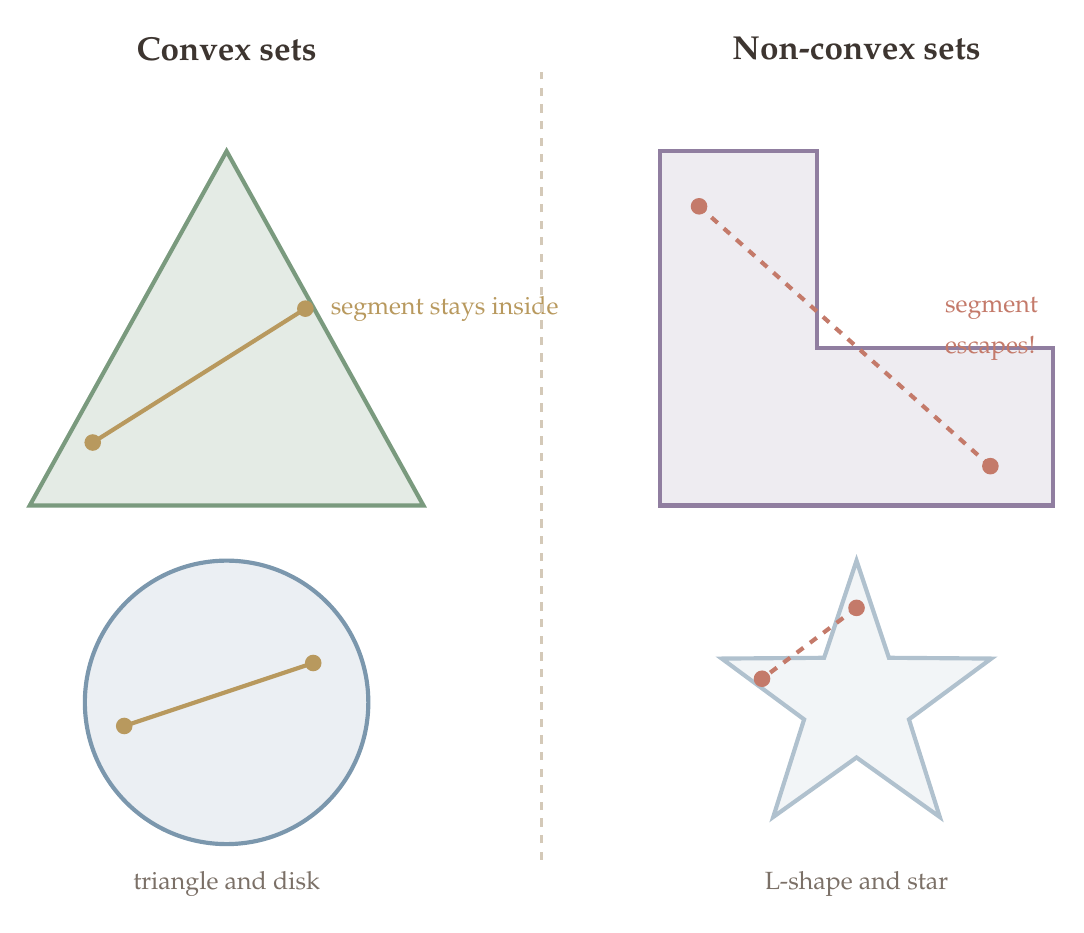
\begin{tikzpicture}[>={Stealth[length=3mm, width=2mm]}]

% --- Left: Convex sets ---
\node[font=\large\bfseries, text=dkbrown] at (3.5,6.8) {Convex sets};

% Triangle (convex)
\fill[sage!20] (1,1) -- (6,1) -- (3.5,5.5) -- cycle;
\draw[sage, line width=1.5pt] (1,1) -- (6,1) -- (3.5,5.5) -- cycle;

% Segment inside
\fill[rwgold] (1.8,1.8) circle (3pt);
\fill[rwgold] (4.5,3.5) circle (3pt);
\draw[rwgold, line width=1.5pt] (1.8,1.8) -- (4.5,3.5);
\node[rwgold, font=\small, anchor=west] at (4.7,3.5) {segment stays inside};

% Disk (convex)
\fill[stblue!15] (3.5,-1.5) circle (1.8);
\draw[stblue, line width=1.5pt] (3.5,-1.5) circle (1.8);

% Segment inside disk
\fill[rwgold] (2.2,-1.8) circle (3pt);
\fill[rwgold] (4.6,-1.0) circle (3pt);
\draw[rwgold, line width=1.5pt] (2.2,-1.8) -- (4.6,-1.0);

\node[wmgray, font=\small] at (3.5,-3.8) {triangle and disk};

% --- Right: Non-convex sets ---
\node[font=\large\bfseries, text=dkbrown] at (11.5,6.8) {Non-convex sets};

% L-shape (non-convex)
\fill[lavender!15] (9,1) -- (14,1) -- (14,3) -- (11,3) -- (11,5.5) -- (9,5.5) -- cycle;
\draw[lavender, line width=1.5pt] (9,1) -- (14,1) -- (14,3) -- (11,3) -- (11,5.5) -- (9,5.5) -- cycle;

% Segment escaping
\fill[terracotta] (9.5,4.8) circle (3pt);
\fill[terracotta] (13.2,1.5) circle (3pt);
\draw[terracotta, line width=1.5pt, dashed] (9.5,4.8) -- (13.2,1.5);

% Mark the part outside
\node[terracotta, font=\small, anchor=west] at (12.5,3.5) {segment};
\node[terracotta, font=\small, anchor=west] at (12.5,3.0) {escapes!};

% 5-pointed star (non-convex): alternating outer (R=1.8) and inner (r=0.7) vertices
\fill[stblue!10]
  ({11.5+1.8*cos(90)},{-1.5+1.8*sin(90)})
  -- ({11.5+0.7*cos(126)},{-1.5+0.7*sin(126)})
  -- ({11.5+1.8*cos(162)},{-1.5+1.8*sin(162)})
  -- ({11.5+0.7*cos(198)},{-1.5+0.7*sin(198)})
  -- ({11.5+1.8*cos(234)},{-1.5+1.8*sin(234)})
  -- ({11.5+0.7*cos(270)},{-1.5+0.7*sin(270)})
  -- ({11.5+1.8*cos(306)},{-1.5+1.8*sin(306)})
  -- ({11.5+0.7*cos(342)},{-1.5+0.7*sin(342)})
  -- ({11.5+1.8*cos(18)},{-1.5+1.8*sin(18)})
  -- ({11.5+0.7*cos(54)},{-1.5+0.7*sin(54)})
  -- cycle;
\draw[stblue!60, line width=1.5pt]
  ({11.5+1.8*cos(90)},{-1.5+1.8*sin(90)})
  -- ({11.5+0.7*cos(126)},{-1.5+0.7*sin(126)})
  -- ({11.5+1.8*cos(162)},{-1.5+1.8*sin(162)})
  -- ({11.5+0.7*cos(198)},{-1.5+0.7*sin(198)})
  -- ({11.5+1.8*cos(234)},{-1.5+1.8*sin(234)})
  -- ({11.5+0.7*cos(270)},{-1.5+0.7*sin(270)})
  -- ({11.5+1.8*cos(306)},{-1.5+1.8*sin(306)})
  -- ({11.5+0.7*cos(342)},{-1.5+0.7*sin(342)})
  -- ({11.5+1.8*cos(18)},{-1.5+1.8*sin(18)})
  -- ({11.5+0.7*cos(54)},{-1.5+0.7*sin(54)})
  -- cycle;

% Segment escaping star (top arm to top-left arm, passes outside through indentation)
\fill[terracotta] (11.5,-0.3) circle (3pt);
\fill[terracotta] (10.3,-1.2) circle (3pt);
\draw[terracotta, line width=1.5pt, dashed] (11.5,-0.3) -- (10.3,-1.2);

\node[wmgray, font=\small] at (11.5,-3.8) {L-shape and star};

% Dividing line
\draw[border, line width=1pt, dashed] (7.5,-3.5) -- (7.5,6.5);

\end{tikzpicture}
\end{document}
